\documentclass[../Thesis.tex]{subfiles}
 
\begin{document}
 
\section  {Preprocessing}
\subsection {Audio Decoding}
..

\subsection {Data Preparation}

The DSD100 dataset must be acquired and added to the project. The dataset consists of 100 full lengths music tracks, and their isolated bass, vocals, drums and accompaniment, all saved under the \texttt{wav} file format. 50 songs are found in the \texttt{dev} folder, meaning there are meant for training, and another 50 are in the \texttt{test} folder, which is meant to use for evaluating. We are actually going to use both for training our model. This will improve it, but will make the tuning phase a little more difficult. To ensure the mixture is a perfect combination of the 2 sources, the mixture will be computed in our code, after the two different wavs are opened. A simple arithmetic mean of the two waveforms will do the trick.

The wavs need to be further translated to the equivalent spectrograms. This will be done using the \texttt{stft} method provided by Librosa. We will be more interested in the magnitude spectra. The phase spectra are not needed for the training phase. They will be used to reconstruct the audios after they are separated, but have no impact on the training of the network. Just another method \texttt{spec\_to\_batch} is required in order to transform the spectra to a batch that can be passed to our model. This method just reshapes and adds padding where needed.


\section {Model}
\subsection {Architecture}

Here we have an overview of the overall architecture for our neural network. As mentioned before, we have decided to use the LSTM variation of the RNN. The network will consist of an input layer, 3 hidden layers with LSTM cells, 2 fully connected (dense) layers and another 2 layers representing the time-frequency masking layer. We will discuss these layers in detail below.
The loss function defined by:  $\mathit{loss} = \mathit{mean}( {( \mathit{y}_{1\mathit{p}} – \mathit{y}_1 )}_{}^2 + {( \mathit{y}_{2\mathit{p}} – \mathit{y}_2 )}_{}^2)$ , 
where: $ \mathit{y}_{1\mathit{p}} $ – predicted source 1 magnitude tensor, $ \mathit{y}_{1} $ – source 1 magnitude tensor, $ \mathit{y}_{2\mathit{p}} $ – predicted source 2 magnitude tensor, $ \mathit{y}_{2} $ – source 2 magnitude tensor 

\begin{figure}[h]
\centering
\label {fig: data_flow}
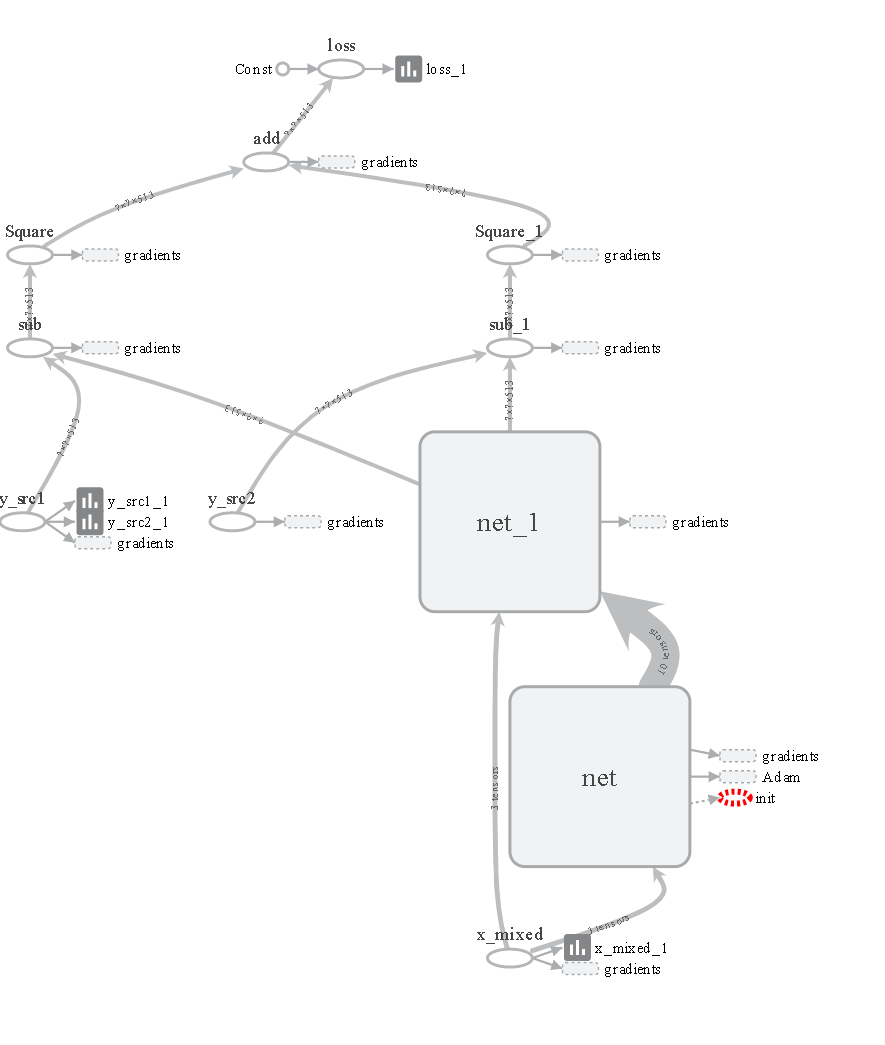
\includegraphics[width=0.5\textwidth]{data_flow.png}
\caption[width=0.5\textwidth]{visualization of the data flow in TensorBoard}
\end{figure}

\begin{figure}[h]
\centering
\label {fig: layers}
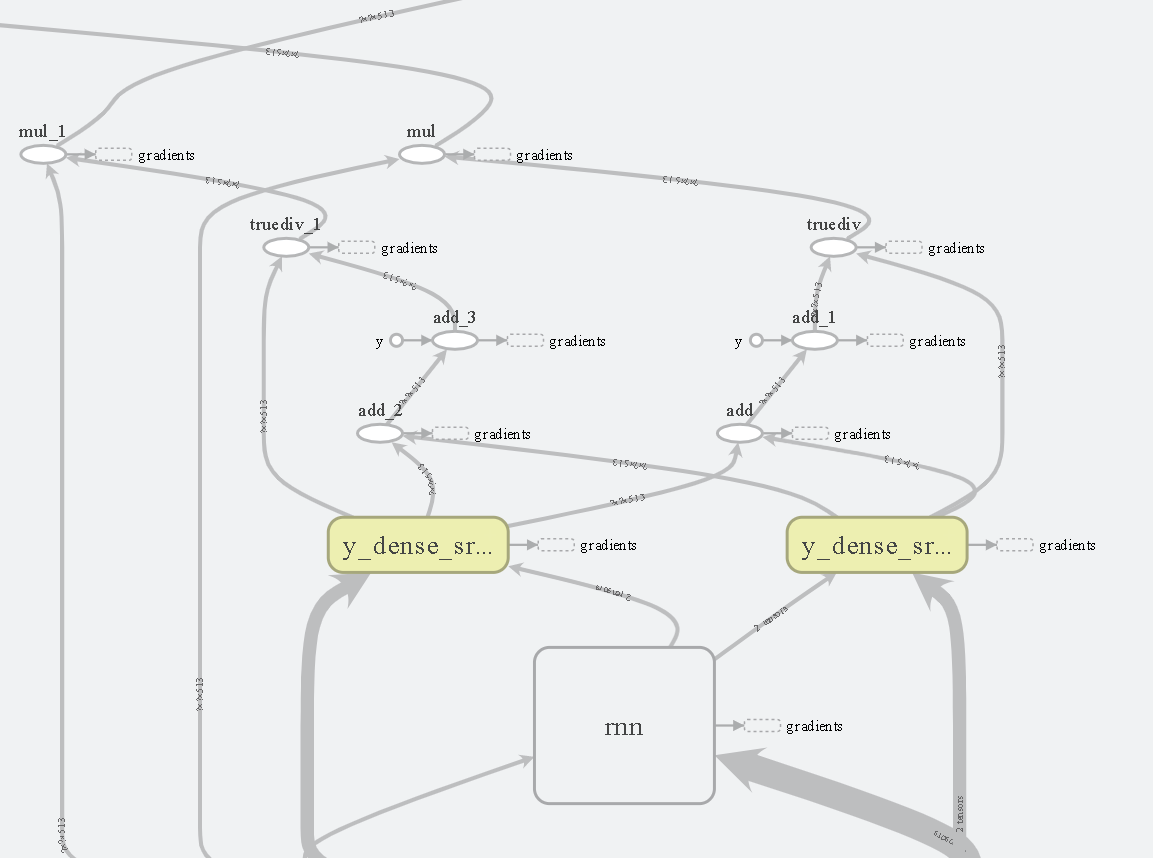
\includegraphics[width=0.5\textwidth]{layers.png}
\caption[width=0.5\textwidth]{LSTM, dense and masking layer viewed in TensorBoard}
\end{figure}

\subsection {Configuration}

Here we will have an overview over the configurable part, and what it represents. Looking at the more important hyperparameters we have: sample rate for the audio files, frame length of the spectrograms, learning rate, checkpoint step and number of seconds of the training audios (batch size). The sample rate is 44100, as the songs are also encoded at this value of Hertz. Frame length of the spectrograms is 1024, the default one using the Librosa package. Learning rate is not fixed. We might start with a 0.001 learning rate and decrease it at about 80\% training, so the model can better tune the features found. Checkpoints should be done as frequently as possible to make sure we aren’t losing progress. This parameter is dependent on the number of training iterations. The batch size is 8.192 seconds. I chose this exact number so we can draw a Mel spectrogram of size 512:512 from the batch if we ever want to visualize the data.

Other objects like session configuration or data path are available in a configuration file. 
We will only train the model to recognize drums and vocals from a mixture of the two. This should be a good start giving the limited time and data available. 


\subsection {Layers}
\subsubsection {Input Layer}

Input layer is composed by a tensor, containing floats, and representing a frame from the magnitude spectrum of the mixture. We create a placeholder for the tensor, using \texttt{tf.placeholder} and call it \texttt{x\_mixed}. We specify one of the dimensions’ size to be equal to half the length of a frame from our spectrogram. This layer is connected to the LSTM layer through edges with trainable weights.

\subsubsection {LSTM Cells}

A configurable number (default 3) of LSTM layers defined. To do this, an LSTM cell must be created for each layer. The size of those cells is hardcoded to 256.To create the LSTM cells we call \texttt{rnn\_cell.LSTM} and provide the mentioned size and to define the layers we use the method \texttt{rnn\_cell.MultiRNNCell} The RNN is created by calling \texttt{tf.nn.dynamic\_rnn}. The input layer will act as input and the LSTM layers defined will act as the core of this network. The output of this network will pass on to two fully connected layers.

\subsubsection {Dense Layer}

Two fully connected layers (one for each source) are formed right after the RNN. These layers will hopefully find patterns that identify each source. It’s important that these two layers are located right after the RNN in order to get information on past data as well.  The number of units is the same as the dimension from the input tensor. A ReLU activation function is associated with these layers, which is perfect for the type of filtering that is done. The method for generating them is \texttt{tf.layers.dense}.


\subsubsection {Time-Freqeuncy Masking Layer}

Two simple time-frequency masking layers will compose the predicted magnitude spectra from the previous dense layers. To obtain those, we divide the dense layer tensor to the sum of the dense layers and multiply it with the input tensor.


\subsubsection {Output}

The output is the two predicted magnitude spectra for our two sources. In the training session, this output is compared to the original sources, in order to compute the loss. In the evaluation session or when we want to obtain the corresponding audio files, these spectra need to be further processed. We define a method to get frequency masks from these magnitudes. These masks are applied to the original mixed magnitude, and are transformed to a waveform. This transformation is done by obtaining the STFT matrix using the stored phase spectra, and further applying the ISTFT to the matrix. We will use the ISTFT implementation provided by Librosa. The resulting waveforms can be written to file.

\subsection {Model Training}

To train our model, we load the model, with the latest state available. Next, we specify the loss method, and the optimizer. After some investigation on this matter, the Adam optimizer was chosen, an implementation being available on TensorFlow. After the initialization, we can start the training session.  Drums and vocals audio are chosen from a random song. From this, only a portion of configurable seconds will be processed. Using the preprocess techniques, we get the corresponding batches for the mixture and the two sources. We pass the loss function, optimizer and the batches to the method run of our current session. This method gets us the loss value, and backpropagates it through our model. In order to save the progress, we will use the checkpoint system implemented in TensorFlow. This lets us save the Variables and parameters of our model and restore them when we restart the software. 

Currently 1000 training iterations are done in about 6 hours. Judging by how the loss value decreases, a satisfiable number of iterations would be around 15.000, which takes over 3 days on this hardware configuration. In order to tune the hyperparameters, multiple individual training session should run. Because of time issues we will research what values these parameters should have and personally observe how it affects our model. No special evaluations are to be done.

\smallskip
Current hardware configuration:

\begin{tabular}{ll}
Processor & i7-7700HQ, \@ 2.80Ghz \\
Physical Memory (RAM) & 8.00 GB  \\
Graphic Card & GTX 1050 4 GB
\end{tabular}

\begin{figure}[h]
\centering
\label {fig: loss}
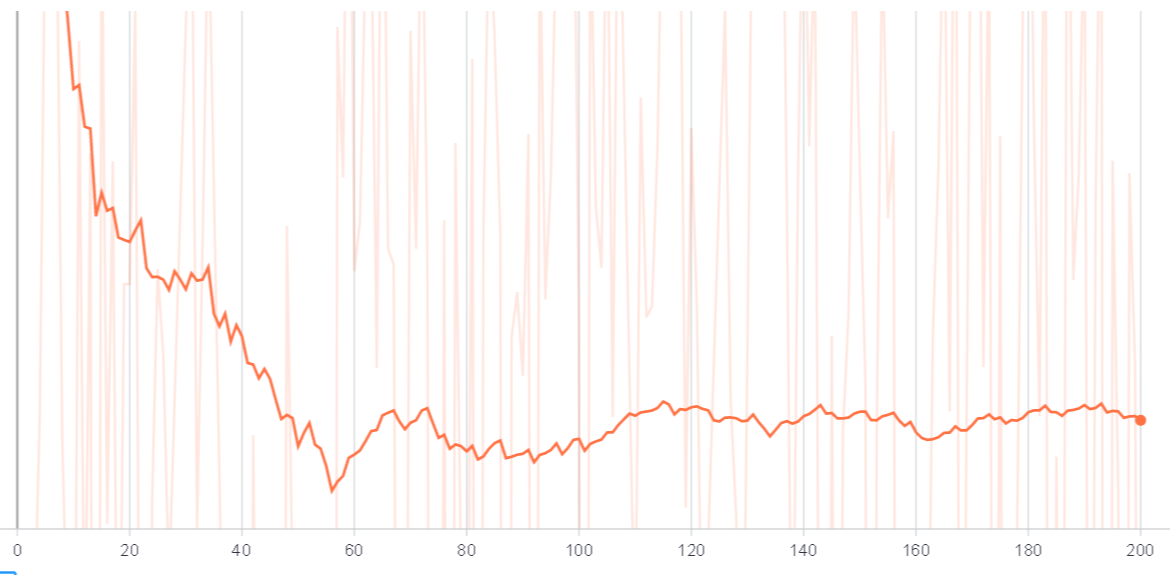
\includegraphics[width=0.5\textwidth]{loss.png}
\caption[width=0.5\textwidth]{Loss value decreasing in time as the model is learning}
\end{figure}

\section {Rest API}
..

\section {Mobile Interface}
..

\section {Web Interface}
..

\end{document}
